\documentclass[aspectratio=169]{beamer}\usepackage[]{graphicx}\usepackage[]{xcolor}
% maxwidth is the original width if it is less than linewidth
% otherwise use linewidth (to make sure the graphics do not exceed the margin)
\makeatletter
\def\maxwidth{ %
  \ifdim\Gin@nat@width>\linewidth
    \linewidth
  \else
    \Gin@nat@width
  \fi
}
\makeatother

\definecolor{fgcolor}{rgb}{0.345, 0.345, 0.345}
\newcommand{\hlnum}[1]{\textcolor[rgb]{0.686,0.059,0.569}{#1}}%
\newcommand{\hlsng}[1]{\textcolor[rgb]{0.192,0.494,0.8}{#1}}%
\newcommand{\hlcom}[1]{\textcolor[rgb]{0.678,0.584,0.686}{\textit{#1}}}%
\newcommand{\hlopt}[1]{\textcolor[rgb]{0,0,0}{#1}}%
\newcommand{\hldef}[1]{\textcolor[rgb]{0.345,0.345,0.345}{#1}}%
\newcommand{\hlkwa}[1]{\textcolor[rgb]{0.161,0.373,0.58}{\textbf{#1}}}%
\newcommand{\hlkwb}[1]{\textcolor[rgb]{0.69,0.353,0.396}{#1}}%
\newcommand{\hlkwc}[1]{\textcolor[rgb]{0.333,0.667,0.333}{#1}}%
\newcommand{\hlkwd}[1]{\textcolor[rgb]{0.737,0.353,0.396}{\textbf{#1}}}%
\let\hlipl\hlkwb

\usepackage{framed}
\makeatletter
\newenvironment{kframe}{%
 \def\at@end@of@kframe{}%
 \ifinner\ifhmode%
  \def\at@end@of@kframe{\end{minipage}}%
  \begin{minipage}{\columnwidth}%
 \fi\fi%
 \def\FrameCommand##1{\hskip\@totalleftmargin \hskip-\fboxsep
 \colorbox{shadecolor}{##1}\hskip-\fboxsep
     % There is no \\@totalrightmargin, so:
     \hskip-\linewidth \hskip-\@totalleftmargin \hskip\columnwidth}%
 \MakeFramed {\advance\hsize-\width
   \@totalleftmargin\z@ \linewidth\hsize
   \@setminipage}}%
 {\par\unskip\endMakeFramed%
 \at@end@of@kframe}
\makeatother

\definecolor{shadecolor}{rgb}{.97, .97, .97}
\definecolor{messagecolor}{rgb}{0, 0, 0}
\definecolor{warningcolor}{rgb}{1, 0, 1}
\definecolor{errorcolor}{rgb}{1, 0, 0}
\newenvironment{knitrout}{}{} % an empty environment to be redefined in TeX

\usepackage{alltt}

% Set lecture number for later use


% Part common to all the lectures
\subtitle{MATH 2740 -- Mathematics of Data Science -- Lecture 01}
\author{\texorpdfstring{Julien Arino\newline\url{julien.arino@umanitoba.ca}}{Julien Arino}}
\institute{Department of Mathematics @ University of Manitoba}

% Title of the lecture
\title{Presentation of the course and setting up R}



\input{slides-setup-whiteBG.tex}

\IfFileExists{upquote.sty}{\usepackage{upquote}}{}
\begin{document}




% Set up cross-references and counter persistence

% Set up cross-references and counter persistence

%%%%%%%%%%%%%%%%%%%%%%%%%%%%%%%%%
%%%%%%%%%%%%%%%%%%%%%%%%%%%%%%%%%
%% TITLE AND OUTLINE
%%%%%%%%%%%%%%%%%%%%%%%%%%%%%%%%%
%%%%%%%%%%%%%%%%%%%%%%%%%%%%%%%%%
\titlepagewithfigure{FIGS-slides-admin/a_robot_looking_at_a_desolate_tree_in_the_style_of_Magritte.png}
\outlinepage{FIGS-slides-admin/a_robot_looking_at_a_desolate_tree_in_the_style_of_Dali.png}


%%%%%%%%%%%%%%%%%%%%
%%%%%%%%%%%%%%%%%%%%
%%%%%%%%%%%%%%%%%%%%
%%%%%%%%%%%%%%%%%%%%
% Some information
\Ssection{General information about the course}{FIGS-slides-admin/a_robot_using_an_easel_to_paint_a_desolate_tree_in_the_style_of_HR_Giger.png}

\begin{frame}{Foreword}
\begin{itemize}
\item "Numerical dates" are in the form YYYY-MM-DD (e.g, these slides were compiled on 2026-09-09)
\vfill
\item Times are 24h (HHMM)
\vfill
\item Units are SI
\end{itemize}
\vfill
In case you want to know, the slides in the course are \code{Rnw} compiled using \code{R}. All (including source code) are available on GitHub \href{https://github.com/julien-arino/math2740-of-data-science}{here}
\end{frame}

\begin{frame}{Getting in touch}
\begin{itemize}
\item \href{mailto:julien.arino@umanitoba.ca}{julien.arino@umanitoba.ca}
\vfill
\item Please use your \texttt{myumanitoba} email address. Use a tag such as \texttt{[MATH 2740]} in your subject line, if you want to be read..
\vfill
\item Word of warning: I am bad with email! I do answer questions after class or during office hours
\end{itemize}
\end{frame}

\begin{frame}{Office hours}
\begin{itemize}
\item Because of the ongoing renovation of Machray Hall, I am sharing an office with 8 other colleagues. Next door are offices shared by another 8 and 4 colleagues
\vfill
\item It is therefore \textbf{impossible} for me to see you in my office
\vfill
\item I have booked 316 St Paul's from 1400 to 1800 on Tuesday for office hours
\vfill
Seeing you outside of office hours is impossible without ample warning, since I actually need to book a room
\end{itemize}
\end{frame}

\begin{frame}{Course website - UMLearn}
\begin{itemize}
\item All information about the course is posted on UMLearn
\vfill
\item It is \textbf{your responsibility} to check the UMLearn site regularly: \textit{Announcements} is how I normally communicate with you about the course
\vfill
\item (Remember to hit the link at the top of the page that says \textit{MATH-2740-A01 - Mathematics of Data Science}, sometimes UMLearn takes you directly to Content, which is not where Announcements are)
\vfill \boldred{Important --} I \textsc{\textbf{do not}} answer emails that ask about things easy to find on UMLearn
\end{itemize}
\end{frame}

\begin{frame}{Lectures}
\begin{itemize}
\item TR 1130--1245 in 100 Fletcher Argue
\vfill
\item Videos for the course as I taught it in 2021 are available as a \href{https://www.youtube.com/playlist?list=PLfRaznSpWo2vQAn1jVyueTuAiryDaxkH3}{YouTube playlist}. There is no guarantee that that the content will be the same this year, but there will be commonalities for sure
\end{itemize}
\end{frame}

\begin{frame}{Tutorials}
\begin{center}
\begin{tabular}{lll}
\toprule
Section & Day and time & Location \\
\midrule
B01 & W 0830--0920 & P230 Duff Roblin \\
B03 & W 0930--1020 & 303 Tier \\
B04 & W 1130--1220 & P230 Duff Roblin \\
\bottomrule
\end{tabular}
\end{center}
\vfill
\begin{itemize}
\item In tutorials, you will review some of the mathematical content and work on computations
\vfill
\item Lab Tests (45 minutes) will be held
\end{itemize}
\end{frame}

\begin{frame}{Evaluation}
\begin{itemize}
\item 3 Lab Tests during tutorials (\textbf{10\%} each for a total \textbf{30\%})
\vfill
\item 1 midterm on Thursday 5 November 2026 1800--2000 (\textbf{35\%})
\vfill
\item 1 final examination during the December 2026 Examination period (\textbf{45\%})
\end{itemize}
\vfill
\begin{itemize}
\item In all written work, explain what you are doing. No explanation $\implies$ lost marks (even if correct)
\end{itemize}
\end{frame}


\begin{frame}{Lab Tests}
\bbullet Held during tutorials on 23 Sept, 21 Oct, 25 Nov
\vfill
\bbullet 45 minutes long 
\vfill
\bbullet You \textbf{must} write Lab Tests in the tutorial you are registered in
\vfill
\bbullet Tests your capacity to do simple proofs or remember definitions or results, as well as computer code
\end{frame}

\begin{frame}{Worksheets}
\begin{itemize}
\item Worksheets will be posted on UM Learn in advance of tutorials
\vfill
\item During the tutorial, the TA will go over some of the problems
\vfill
\item Worksheets are NOT for credit; they are meant as extra practice
\vfill
\item Lab Tests, the Midterm and Final Examinations will all contain one question asking you to explain what a piece of code does
\end{itemize}
\end{frame}


\begin{frame}{Self-declaration of absences}
\begin{itemize}
\item You can self-declare an absence of less than 120 hours (5 days)
\vfill
\item Self-declarations are intended for occasional and unforeseen circumstances $\implies$ I \textbf{will not accept more than one} during the term
\vfill
\item Self-declarations must be filed less than 48 hours after the event you are using it for
\vfill
\item There is no make up for anything missed because of a self-declared absence: any percentage will be moved to the final examination
\vfill
\item See the details and the form here (\href{https://umanitoba.ca/student-supports/academic-supports/student-advocacy/self-declaration-policy-students}{link}). You \textbf{must} use the form on that page to self-declare your absence
\end{itemize}
\end{frame}

\begin{frame}{Definitions are colour coded}
Memorising the definitions is part of the course. To help, definitions are colour coded
\vfill
\begin{definition}[Definitions]
These definitions are important, you need to know them
\end{definition}
\vfill
\begin{minordefinition}[Less important definitions]
These definitions are a little less important, you will not be asked to state them (although it is a good idea to know them anyway)
\end{minordefinition}
\end{frame}

\begin{frame}{Results are colour coded}
Memorising some of the results is part of the course. To help, results are colour coded
\vfill
\begin{theorem}[Theorems]
Theorems in blue boxes are worth knowing but you will not be asked to reproduce them
\end{theorem}
\vfill
\begin{importanttheorem}[Important theorems]  
Theorems in red boxes are important, you should know them and be able to reproduce them
\end{importanttheorem}
\end{frame}


\begin{frame}[red]{You must know how to do some proofs}
There are a few proofs (not many!) that I want you to know how to do
\vfill
Such proofs appear on slides like the present one, with a red background
\end{frame}


%%%%%%%%%%%%%%%%%%%%
%%%%%%%%%%%%%%%%%%%%
%%%%%%%%%%%%%%%%%%%%
%%%%%%%%%%%%%%%%%%%%
% Some information
\Ssection{Mathematics of data science?}{FIGS-slides-admin/Gemini_Generated_Image_uwh6druwh6druwh6.jpeg}

\begin{frame}{In days of yore (circa 2010)}
\begin{quote}
Big data is like teenage sex: everyone talks about it, nobody really knows how to do it, everyone thinks everyone else is doing it, so everyone claims they are doing it...
\end{quote}

Attributed to \href{https://twitter.com/danariely/status/287952257926971392?lang=en}{Dan Ariely} (Duke University)
\vfill
The vocabulary has evolved, big data $\to$ complex data $\to$ data science, but Data Science remains a loosely defined concept, although things are becoming better
\end{frame}

\begin{frame}{Data Science (according to Wikipedia)}
Data science is an \textbf{interdisciplinary field} that uses scientific methods, processes, algorithms and systems to extract knowledge and insights from \textbf{structured} and \textbf{unstructured data}, and apply knowledge and actionable insights from data across a broad range of application domains.
\vfill
[..] It uses techniques and theories drawn from many fields within the context of \textbf{mathematics}, \textbf{statistics}, \textbf{computer science}, \textbf{information science}, and \textbf{domain knowledge}.
\end{frame}

\begin{frame}{The data deluge}
\bbullet Data science is nothing new (some statisticians argue it is just another name for statistics), but it has become prominent in recent years as a consequence of the unprecedented mass of information generated and collected by our modern societies
\vfill
\bbullet One speaks of \textit{information explosion} or \textit{data deluge}. See some considerations, e.g., \href{https://bernardmarr.com/how-much-data-is-there-in-the-world/}{here}
\end{frame}

\begin{frame}{A wide variety of jobs}
We have absolutely insane amounts of data and we try to make sense of it
\vfill
$\implies$ data science
\vfill
However, except for the name, the situation has not improved significantly since the days of yore of Ariely's quote: data science is a hodge-podge that contains everything but the kitchen sink
\vfill
To caricature
\begin{itemize}
\item two main types of data: structured and unstructured
\item two main branches: statistics and computer science
\item two main types of jobs: users and developpers
\end{itemize}
\end{frame}

\begin{frame}{\textit{Math} of Data Science?}
\begin{itemize}
\item DS has two main branches: statistics and computer science
\item DS has two main types of jobs: users and developpers
\end{itemize}
\vfill
So why a course on Math of Data Science?
\vfill
If you plan to be a user and are not curious about \textit{the how} and \textit{the why} and can tolerate errors due to misuse of methods, then you probably don't care about this course
\vfill
In other cases, many of the concepts used have their roots in math and to understand where the methods are coming from and, even more importantly, to develop new methods, math is often required
\end{frame}

\begin{frame}{Warning! We barely brush the surface}
\begin{itemize}
\item Some techniques from linear algebra
\vfill
\item Some graph theory ideas
\vfill
\item A little bit of multivariable calculus
\end{itemize}
\vfill
There is a lot more to see!!!
\end{frame}

\begin{frame}{Prerequisites / What you will learn}
\bbullet (MATH 1210 or MATH 1220 or MATH 1300) and (MATH 1232 or MATH 1700 or MATH 1710)
\vfill
$\Rightarrow$ You \textbf{must know and be comfortable} with 1st year linear algebra (3 CH) and 1st year calculus (6 CH)
\vfill
\bbullet We need more: some stuff you would learn in 2090 (Linear Algebra 2), some stuff from 2130, 2150 or 2720 (Multivariable Calculus) and some stuff from 2070 (Graph Theory)
\end{frame}

\begin{frame}{Focus here is not on mathematical ``precision''}
\bbullet We won't do complicated proofs. I will show some when they are useful in understanding \textit{why} something works
\vfill
\bbullet We will cover just enough of the mentioned math topics that you can understand \textit{how} to do things
\vfill
\bbullet In classic math courses, we work on ``small'' examples so we can work them by hand and are able to do them in tests
\vfill
Here, we will do small examples by hand, indeed. But you will do regularly sized examples in computer assignments
\end{frame}


%%%%%%%%%%%%%%%%%%%%
%%%%%%%%%%%%%%%%%%%%
%%%%%%%%%%%%%%%%%%%%
%%%%%%%%%%%%%%%%%%%%
\Ssection{Setting things up for the course}{FIGS-slides-admin/Gemini_Generated_Image_4vlmzf4vlmzf4vlm.jpeg}

\begin{frame}{We will be programming quite a bit}
As already indicated, Data Science is a very hands-on discipline. We will be programming quite a bit in this course
\vfill
Indeed, we can work out some of the examples "by hand", but to make things interesting, we typically need to consider larger examples where hand calculations are not pleasant or not even feasible
\end{frame}

\begin{frame}{R versus Python}
Slightly different take on life :)
\vfill
In short: \texttt{Python} is more CS, \texttt{R} is more Stats/Math
\vfill
Both are good languages for data science
\vfill
In this course, assignments \textbf{must} use \texttt{R}
\end{frame}

\begin{frame}{R was originally for stats but is now more}
\begin{itemize}
\item Open source version of S
\vfill
\item Appeared in 1993
\vfill
\item Now version 4.5
\vfill
\item Uses a lot of C and Fortran code. E.g., \texttt{deSolve}:
\begin{quote}
The functions provide an interface to the FORTRAN functions 'lsoda', 'lsodar', 'lsode', 'lsodes' of the 'ODEPACK' collection, to the FORTRAN functions 'dvode', 'zvode' and 'daspk' and a C-implementation of solvers of the 'Runge-Kutta' family with fixed or variable time steps
\end{quote}
\vfill
\item Very active community on the web, easy to find solutions \end{itemize}
\end{frame}

\begin{frame}{Getting your computer ready for the course}
All computer coding is in \texttt{R}; assignments also need to be returned in \texttt{R}
\vfill
$\implies$ you need to find a way to run \texttt{R}. Next slide: some methods, from the easiest to the most challenging.
\vfill
Note that all options described below are Open Source (completely free)
\end{frame}

\begin{frame}{In short...}
\begin{itemize}
\item Terminal version, not very friendly
\vfill
\item Nicer terminal: \href{https://github.com/randy3k/radian}{radian}
\vfill
\item Execute R scripts by using \texttt{Rscript name\_of\_script.R}. Useful to run code in \texttt{cron}, for instance
\vfill
\item Use IDEs:
    \begin{itemize}
    \item \href{https://www.rstudio.com/products/rstudio/}{RStudio} has become the reference
    \item \href{https://invent.kde.org/education/rkward}{RKWard} is useful if you are for instance using an ARM processor (Raspberry Pi, some Chromebooks..)
    \end{itemize}
\vfill
\item Integrate into jupyter notebooks
\end{itemize}
\end{frame}

\begin{frame}{Install R and RStudio}
This is probably the best option if you intend to go a little further than what we will do in the course. \texttt{R} is available on most platforms, while \texttt{RStudio} is available on most platforms except for Linux ARM devices (but can be compiled there)
\vfill
Visit \href{https://www.r-project.org/}{https://www.r-project.org/}
\vfill
Choose your version: Windows or Mac. Under Linux, you can install directly from your package manager (e.g., \texttt{sudo apt install R-base} for Debian-based distros)
\vfill
To install RStudio, see \href{https://www.rstudio.com/products/rstudio/}{here}
\end{frame}

\begin{frame}{Going further}
\begin{itemize}
\item \href{https://www.rstudio.com/products/rstudio/\#rstudio-server}{RStudio server}: run RStudio on a Linux server and connect via a web interface
\vfill
\item Shiny: easily create an interactive web site running R code
\vfill
\item \href{https://www.rstudio.com/products/shiny/shiny-server/}{Shiny server}: run Shiny apps on a Linux server
\vfill
\item Rmarkdown: markdown that incorporates R commands. Useful for generating reports in html or pdf, can make slides as well..
\vfill
\item Sweave/knitr: \LaTeX\ incorporating R commands. Useful for generating reports. Not used as much as Rmarkdown these days (but used for these slides)
\end{itemize}
\end{frame}


%%%%%%%%%%%%%%%%%%%%
%%%%%%%%%%%%%%%%%%%%
%%%%%%%%%%%%%%%%%%%%
%%%%%%%%%%%%%%%%%%%%
% Some information
\Ssection{Introduction to R Markdown}{FIGS-slides-admin/Gemini_Generated_Image_pbzl1mpbzl1mpbzl.jpeg}



\begin{frame}
  \frametitle{R Markdown?}
  \begin{itemize}
    \item File format for making dynamic documents with R
    \vfill
    \item Combines code, its results and narrative text in a single document
    \vfill
    \item Uses simple \code{Markdown} syntax for text and \code{R} code chunks for analysis
    \vfill
    \item From one `.Rmd` file, you can create HTML, PDF, Word documents, presentations, ...
  \end{itemize}
\end{frame}

\begin{frame}[fragile]
  \frametitle{The YAML header}
Every R Markdown document starts with a YAML header, enclosed by \code{---}. This controls the overall properties of the document
\begin{block}{Example YAML for a PDF document}
\begin{verbatim}
---
title: "My Report"
author: "My Name"
date: "2025-08-17"
output:
  pdf_document:
    toc: true
    number_sections: true
---
\end{verbatim}
\end{block}
\end{frame}

\begin{frame}[fragile]
  \frametitle{Basic Text Formatting}
  Markdown provides a simple syntax for formatting text
  \vfill
  \begin{itemize}
    \item \verb|# Header| creates a section title, \verb|## Sub-header| creates a subsection title, etc.
    \vfill
    \item \verb|*italic text*| produces \textit{italic text}
    \vfill
    \item \verb|**bold text**| produces \textbf{bold text}
    \vfill
    \item \verb|`code font`| produces \texttt{code font}
  \end{itemize}
\end{frame}

\begin{frame}[fragile]{Lists}
Unordered lists start with \verb|*| or \verb|-|
\begin{verbatim}
* Item 1
* Item 2
\end{verbatim}
\vfill
Ordered lists use numbers
\begin{verbatim}
1. First Item
2. Second Item
\end{verbatim}
\vfill
(Once the numbered list is ``initiated'', the number doesn't matter, you can write 1., 1., 1., etc., provided you have a new line each time)
\end{frame}

\begin{frame}[fragile]
  \frametitle{Chunks: the core of R Markdown}
  R code is placed in ``chunks'', which start with \verb|```{r chunk-name}| and end with \verb|```|
\begin{lstlisting}
```{r cars-summary}
# Your R code goes here
summary(cars)
```
\end{lstlisting}
\vfill
Chunk names (\code{cars-summary} here) are not mandatory (you could write \code{```\{r\}} but are very useful, in particular when debugging
\end{frame}

\begin{frame}[fragile]
  \frametitle{Chunk output}
  When the document is "knit," the \code{R} code is executed and its output is embedded in the final document
\begin{lstlisting}
```{r cars-summary}
summary(cars)
```
\end{lstlisting}
\begin{knitrout}
\definecolor{shadecolor}{rgb}{0.969, 0.969, 0.969}\color{fgcolor}\begin{kframe}
\begin{verbatim}
##      speed           dist       
##  Min.   : 4.0   Min.   :  2.00  
##  1st Qu.:12.0   1st Qu.: 26.00  
##  Median :15.0   Median : 36.00  
##  Mean   :15.4   Mean   : 42.98  
##  3rd Qu.:19.0   3rd Qu.: 56.00  
##  Max.   :25.0   Max.   :120.00
\end{verbatim}
\end{kframe}
\end{knitrout}
\end{frame}

\begin{frame}[fragile]
  \frametitle{Controlling chunks with options}
  Chunk behavior is controlled by options inside the curly braces
  \vfill
  \begin{itemize}
    \item \verb|echo=FALSE| hides the \code{R} code, but shows the output
    \vfill
    \item \verb|eval=FALSE| shows the code, but does not execute it
    \vfill
    \item \verb|include=FALSE| executes the code, but hides both code and output
    \vfill
    \item \verb|warning=FALSE|, \verb|message=FALSE| hides warnings or messages
    \vfill
    \item \verb|fig.width=5|, \verb|fig.height=4| sets figure dimensions
  \end{itemize}
\end{frame}

\begin{frame}[fragile]
  \frametitle{Figure chunks}
  Plots are automatically embedded
\begin{lstlisting}
```{r pressure-plot, echo=FALSE, fig.cap="Pressure Data"}
plot(pressure)
```
\end{lstlisting}

\begin{center}
% We cheat, of course, as this is Rnw not Rmd..
\begin{knitrout}
\definecolor{shadecolor}{rgb}{0.969, 0.969, 0.969}\color{fgcolor}
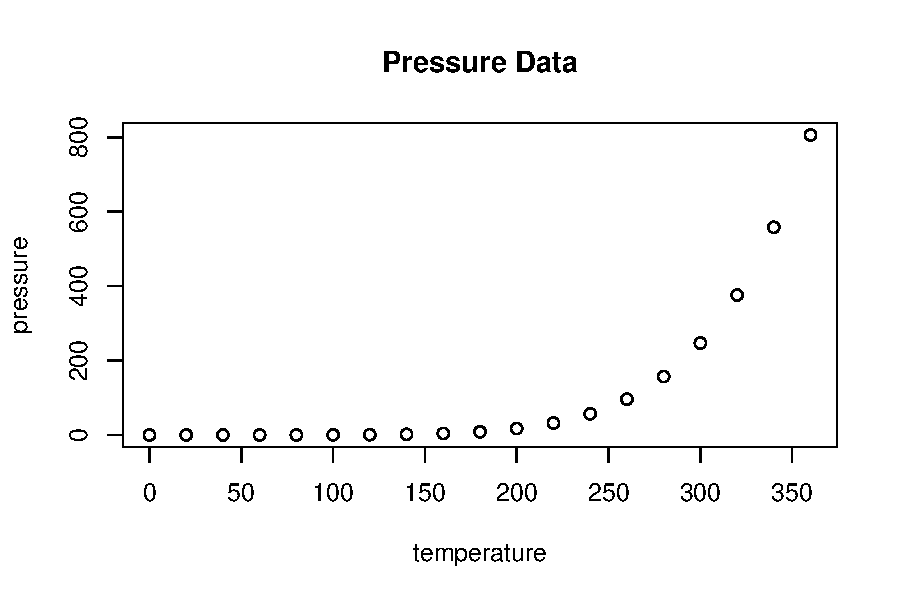
\includegraphics[width=0.65\textwidth]{FIGS/L01-pressure-plot-rmd-1} 
\end{knitrout}
\end{center}
\end{frame}

\begin{frame}[fragile]
  \frametitle{Inline R Code}
  You can embed \code{R} code directly into text with backticks: \verb|`r ...`|
  \vfill
\begin{lstlisting}
The `cars` dataset has `r nrow(cars)` rows.
\end{lstlisting}
  \vfill
  The \code{cars} dataset has 50 rows.
\end{frame}

%%%%%%%%%%%%%%%%%%%%
%%%%%%%%%%%%%%%%%%%%
%%%%%%%%%%%%%%%%%%%%
%%%%%%%%%%%%%%%%%%%%
\Ssection{(Super brief) Introduction to programming in R}{FIGS-slides-admin/Gemini_Generated_Image_dzsfcndzsfcndzsf.jpeg}

\begin{frame}{R is a scripted language}
\begin{itemize}
\item Interactive
\vfill
\item Allows you to work in real time
\vfill
    \begin{itemize}
    \item Be careful: what is in memory might involve steps not written down in a script
    \vfill
    \item If you want to reproduce your steps, it is good to write all the steps down in a script and to test from time to time running using \texttt{Rscript}: this will ensure that all that is required to run is indeed loaded to memory when it needs to, i.e., that it is not already there..
    \end{itemize}
\end{itemize}
\end{frame}


\begin{frame}{Assignment}
Two ways:

\begin{knitrout}
\definecolor{shadecolor}{rgb}{0.969, 0.969, 0.969}\color{fgcolor}\begin{kframe}
\begin{alltt}
\hldef{X} \hlkwb{<-} \hlnum{10}
\end{alltt}
\end{kframe}
\end{knitrout}

or

\begin{knitrout}
\definecolor{shadecolor}{rgb}{0.969, 0.969, 0.969}\color{fgcolor}\begin{kframe}
\begin{alltt}
\hldef{X} \hlkwb{=} \hlnum{10}
\end{alltt}
\end{kframe}
\end{knitrout}

First version is preferred by R purists.. I don't really care
\end{frame}

\begin{frame}[fragile]{Lists}
A very useful data structure, quite flexible and versatile. Empty list: \texttt{L <- list()}. Convenient for things like parameters. For instance

\begin{knitrout}
\definecolor{shadecolor}{rgb}{0.969, 0.969, 0.969}\color{fgcolor}\begin{kframe}
\begin{alltt}
\hldef{L} \hlkwb{<-} \hlkwd{list}\hldef{()}
\hldef{L}\hlopt{$}\hldef{a} \hlkwb{<-} \hlnum{10}
\hldef{L}\hlopt{$}\hldef{b} \hlkwb{<-} \hlnum{3}
\hldef{L[[}\hlsng{"another_name"}\hldef{]]} \hlkwb{<-} \hlsng{"Plouf plouf"}
\end{alltt}
\end{kframe}
\end{knitrout}
\end{frame}

\begin{frame}[fragile]
\begin{knitrout}
\definecolor{shadecolor}{rgb}{0.969, 0.969, 0.969}\color{fgcolor}\begin{kframe}
\begin{alltt}
\hldef{L[}\hlnum{1}\hldef{]}
\end{alltt}
\begin{verbatim}
## $a
## [1] 10
\end{verbatim}
\begin{alltt}
\hldef{L[[}\hlnum{2}\hldef{]]}
\end{alltt}
\begin{verbatim}
## [1] 3
\end{verbatim}
\begin{alltt}
\hldef{L}\hlopt{$}\hldef{a}
\end{alltt}
\begin{verbatim}
## [1] 10
\end{verbatim}
\begin{alltt}
\hldef{L[[}\hlsng{"b"}\hldef{]]}
\end{alltt}
\begin{verbatim}
## [1] 3
\end{verbatim}
\begin{alltt}
\hldef{L}\hlopt{$}\hldef{another_name}
\end{alltt}
\begin{verbatim}
## [1] "Plouf plouf"
\end{verbatim}
\end{kframe}
\end{knitrout}
\end{frame}

\begin{frame}[fragile]{Vectors}
\begin{knitrout}
\definecolor{shadecolor}{rgb}{0.969, 0.969, 0.969}\color{fgcolor}\begin{kframe}
\begin{alltt}
\hldef{x} \hlkwb{=} \hlnum{1}\hlopt{:}\hlnum{10}
\hldef{y} \hlkwb{<-} \hlkwd{c}\hldef{(x,} \hlnum{12}\hldef{)}
\hldef{y}
\hldef{z} \hlkwb{=} \hlkwd{c}\hldef{(}\hlsng{"red"}\hldef{,} \hlsng{"blue"}\hldef{)}
\hldef{z}
\hldef{z} \hlkwb{=} \hlkwd{c}\hldef{(z,} \hlnum{1}\hldef{)}
\hldef{z}
\end{alltt}
\end{kframe}
\end{knitrout}

Note that in \texttt{z}, since the first two entries are characters, the added entry is also a character. Contrary to lists, vectors have all entries of the same type
\end{frame}

\begin{frame}[fragile]{Matrices}
Matrix (or vector) of zeros
\begin{knitrout}
\definecolor{shadecolor}{rgb}{0.969, 0.969, 0.969}\color{fgcolor}\begin{kframe}
\begin{alltt}
\hldef{A} \hlkwb{<-} \hlkwd{mat.or.vec}\hldef{(}\hlkwc{nr} \hldef{=} \hlnum{2}\hldef{,} \hlkwc{nc} \hldef{=} \hlnum{3}\hldef{)}
\hldef{A}
\end{alltt}
\begin{verbatim}
##      [,1] [,2] [,3]
## [1,]    0    0    0
## [2,]    0    0    0
\end{verbatim}
\end{kframe}
\end{knitrout}
\end{frame}


\begin{frame}[fragile]{Matrix are column-first}
\begin{knitrout}
\definecolor{shadecolor}{rgb}{0.969, 0.969, 0.969}\color{fgcolor}\begin{kframe}
\begin{alltt}
\hldef{B} \hlkwb{<-} \hlkwd{matrix}\hldef{(}\hlkwd{c}\hldef{(}\hlnum{1}\hldef{,}\hlnum{2}\hldef{,}\hlnum{3}\hldef{,}\hlnum{4}\hldef{),} \hlkwc{nr} \hldef{=} \hlnum{2}\hldef{,} \hlkwc{nc} \hldef{=} \hlnum{2}\hldef{)}
\hldef{B}
\end{alltt}
\begin{verbatim}
##      [,1] [,2]
## [1,]    1    3
## [2,]    2    4
\end{verbatim}
\begin{alltt}
\hldef{C} \hlkwb{<-} \hlkwd{matrix}\hldef{(}\hlkwd{c}\hldef{(}\hlnum{1}\hldef{,}\hlnum{2}\hldef{,}\hlnum{3}\hldef{,}\hlnum{4}\hldef{),} \hlkwc{nr} \hldef{=} \hlnum{2}\hldef{,} \hlkwc{nc} \hldef{=} \hlnum{2}\hldef{,} \hlkwc{byrow} \hldef{=} \hlnum{TRUE}\hldef{)}
\hldef{C}
\end{alltt}
\begin{verbatim}
##      [,1] [,2]
## [1,]    1    2
## [2,]    3    4
\end{verbatim}
\end{kframe}
\end{knitrout}

Remark that here and elsewhere, naming the arguments (e.g., \texttt{nr = 2}) allows to use arguments in any order
\end{frame}

\begin{frame}{Matrix operations}
Probably the biggest annoyance in R compared to other languages
\vfill
\begin{itemize}
\item The notation \texttt{A*B} is the \textit{Hadamard product} $A\circ B$ (what would be denoted \texttt{A.*B} in matlab), not the standard matrix multiplication
\vfill
\item Matrix multiplication is written \texttt{A \%*\% B}
\end{itemize}
\end{frame}

\begin{frame}[fragile]{Vector operations}
Vector addition is also frustrating. Say you create the vector
\begin{knitrout}
\definecolor{shadecolor}{rgb}{0.969, 0.969, 0.969}\color{fgcolor}\begin{kframe}
\begin{alltt}
\hldef{x} \hlkwb{=} \hlnum{1}\hlopt{:}\hlnum{10}
\hldef{x}
\end{alltt}
\begin{verbatim}
##  [1]  1  2  3  4  5  6  7  8  9 10
\end{verbatim}
\end{kframe}
\end{knitrout}

Then \texttt{x+1} gives
\begin{knitrout}
\definecolor{shadecolor}{rgb}{0.969, 0.969, 0.969}\color{fgcolor}\begin{kframe}
\begin{alltt}
\hldef{x}\hlopt{+}\hlnum{1}
\end{alltt}
\begin{verbatim}
##  [1]  2  3  4  5  6  7  8  9 10 11
\end{verbatim}
\end{kframe}
\end{knitrout}

i.e., adds 1 to all entries in the vector.
Beware of this in particular when addressing sets of indices in lists, vectors or matrices
\end{frame}

\begin{frame}[fragile]{Flow control}
\begin{knitrout}
\definecolor{shadecolor}{rgb}{0.969, 0.969, 0.969}\color{fgcolor}\begin{kframe}
\begin{alltt}
\hlkwd{if} (condition is true) \{
  list of stuff to do
\}
\end{alltt}
\end{kframe}
\end{knitrout}

Even if \texttt{list of stuff to do} is a single instruction, best to use curly braces

\begin{knitrout}
\definecolor{shadecolor}{rgb}{0.969, 0.969, 0.969}\color{fgcolor}\begin{kframe}
\begin{alltt}
\hlkwd{if} (condition is true) \{
  list of stuff to do
\} else \hlkwd{if} (another condition) \{
  ...
\} else \{
  ...
\}
\end{alltt}
\end{kframe}
\end{knitrout}
\end{frame}

\begin{frame}[fragile]{For loops}
\texttt{for} applies to lists or vectors

\begin{knitrout}
\definecolor{shadecolor}{rgb}{0.969, 0.969, 0.969}\color{fgcolor}\begin{kframe}
\begin{alltt}
\hlkwd{for} (i in 1:10) \{
  something using integer i
\}
\hlkwd{for} (j in \hlkwd{c}(1,3,4)) \{
  something using integer j
\}
\hlkwd{for} (n in \hlkwd{c}(\hlsng{"truc"}, \hlsng{"muche"}, \hlsng{"chose"})) \{
  something using string n
\}
\hlkwd{for} (m in \hlkwd{list}(\hlsng{"truc"}, \hlsng{"muche"}, \hlsng{"chose"}, 1, 2)) \{
  something using string n or integer n, depending
\}
\end{alltt}
\end{kframe}
\end{knitrout}
\end{frame}

\begin{frame}[fragile]{lapply}
Very useful function (a few others in the same spirit: \texttt{sapply}, \texttt{vapply}, \texttt{mapply})

Applies a function to each entry in a list/vector/matrix. Because there is a parallel version (\texttt{parLapply}) that we will see later, worth learning

\begin{knitrout}
\definecolor{shadecolor}{rgb}{0.969, 0.969, 0.969}\color{fgcolor}\begin{kframe}
\begin{alltt}
\hldef{l} \hlkwb{=} \hlkwd{list}\hldef{()}
\hlkwa{for} \hldef{(i} \hlkwa{in} \hlnum{1}\hlopt{:}\hlnum{10}\hldef{) \{}
        \hldef{l[[i]]} \hlkwb{=} \hlkwd{runif}\hldef{(i)}
\hldef{\}}
\hlkwd{lapply}\hldef{(}\hlkwc{X} \hldef{= l,} \hlkwc{FUN} \hldef{= mean)}
\end{alltt}
\end{kframe}
\end{knitrout}

or, to make a vector

\begin{knitrout}
\definecolor{shadecolor}{rgb}{0.969, 0.969, 0.969}\color{fgcolor}\begin{kframe}
\begin{alltt}
\hlkwd{unlist}\hldef{(}\hlkwd{lapply}\hldef{(}\hlkwc{X} \hldef{= l,} \hlkwc{FUN} \hldef{= mean))}
\end{alltt}
\end{kframe}
\end{knitrout}

or

\begin{knitrout}
\definecolor{shadecolor}{rgb}{0.969, 0.969, 0.969}\color{fgcolor}\begin{kframe}
\begin{alltt}
\hlkwd{sapply}\hldef{(}\hlkwc{X} \hldef{= l,} \hlkwc{FUN} \hldef{= mean)}
\end{alltt}
\end{kframe}
\end{knitrout}
\end{frame}

\begin{frame}[fragile]{``Advanced'' lapply}
Can ``pick up'' nontrivial list entries

\begin{knitrout}
\definecolor{shadecolor}{rgb}{0.969, 0.969, 0.969}\color{fgcolor}\begin{kframe}
\begin{alltt}
\hldef{l} \hlkwb{=} \hlkwd{list}\hldef{()}
\hlkwa{for} \hldef{(i} \hlkwa{in} \hlnum{1}\hlopt{:}\hlnum{10}\hldef{) \{}
        \hldef{l[[i]]} \hlkwb{=} \hlkwd{list}\hldef{()}
        \hldef{l[[i]]}\hlopt{$}\hldef{a} \hlkwb{=} \hlkwd{runif}\hldef{(i)}
        \hldef{l[[i]]}\hlopt{$}\hldef{b} \hlkwb{=} \hlkwd{runif}\hldef{(}\hlnum{2}\hlopt{*}\hldef{i)}
\hldef{\}}
\hlkwd{sapply}\hldef{(}\hlkwc{X} \hldef{= l,} \hlkwc{FUN} \hldef{=} \hlkwa{function}\hldef{(}\hlkwc{x}\hldef{)} \hlkwd{length}\hldef{(x}\hlopt{$}\hldef{b))}
\end{alltt}
\end{kframe}
\end{knitrout}

gives

\begin{knitrout}
\definecolor{shadecolor}{rgb}{0.969, 0.969, 0.969}\color{fgcolor}\begin{kframe}
\begin{alltt}
\hlcom{# [1]  2  4  6  8 10 12 14 16 18 20}
\end{alltt}
\end{kframe}
\end{knitrout}

Just recall: the argument to the function you define is a list entry (\texttt{l[[1]]}, \texttt{l[[2]]}, etc., here)
\end{frame}

\begin{frame}[fragile]{Avoid parameter variation loops with expand.grid}
\begin{knitrout}
\definecolor{shadecolor}{rgb}{0.969, 0.969, 0.969}\color{fgcolor}\begin{kframe}
\begin{alltt}
\hlcom{# Suppose we want to vary 3 parameters}
\hldef{variations} \hlkwb{=} \hlkwd{list}\hldef{(}
    \hlkwc{p1} \hldef{=} \hlkwd{seq}\hldef{(}\hlnum{1}\hldef{,} \hlnum{10}\hldef{,} \hlkwc{length.out} \hldef{=} \hlnum{10}\hldef{),}
    \hlkwc{p2} \hldef{=} \hlkwd{seq}\hldef{(}\hlnum{0}\hldef{,} \hlnum{1}\hldef{,} \hlkwc{length.out} \hldef{=} \hlnum{10}\hldef{),}
    \hlkwc{p3} \hldef{=} \hlkwd{seq}\hldef{(}\hlopt{-}\hlnum{1}\hldef{,} \hlnum{1}\hldef{,} \hlkwc{length.out} \hldef{=} \hlnum{10}\hldef{)}
\hldef{)}

\hlcom{# Create the list}
\hldef{tmp} \hlkwb{=} \hlkwd{expand.grid}\hldef{(variations)}
\hldef{PARAMS} \hlkwb{=} \hlkwd{list}\hldef{()}
\hlkwa{for} \hldef{(i} \hlkwa{in} \hlnum{1}\hlopt{:}\hlkwd{dim}\hldef{(tmp)[}\hlnum{1}\hldef{]) \{}
    \hldef{PARAMS[[i]]} \hlkwb{=} \hlkwd{list}\hldef{()}
    \hlkwa{for} \hldef{(k} \hlkwa{in} \hlnum{1}\hlopt{:}\hlkwd{length}\hldef{(variations)) \{}
        \hldef{PARAMS[[i]][[}\hlkwd{names}\hldef{(variations)[k]]]} \hlkwb{=} \hldef{tmp[i, k]}
    \hldef{\}}
\hldef{\}}
\end{alltt}
\end{kframe}
\end{knitrout}

There is still a loop, but you can split this list, use it on different machines, etc. And can use \texttt{parLapply}
\end{frame}


%%%%%%%%%%%%%%%%%%%%%%%
%%%%%%%%%%%%%%%%%%%%%%%
%%%%%%%%%%%%%%%%%%%%%%%
%%%%%%%%%%%%%%%%%%%%%%%
\section*{Final remarks}
\begin{frame}\frametitle{Can I have this wrapped up to go?}
For each slide set including \code{R} code, we generate an \code{R} file in the \code{CODE} directory with all the code chunks in this \code{Rnw} file and no \LaTeX
\vfill
% Convert the file to R code. 
% Only include if including R code in the document,
% otherwise it will generate a meaningless file with just 
% and knitr options.

Source the file (if you are reading \code{SLIDES/filename.pdf}, then you want \code{CODE/filename.R}) to reproduce all results in the slide set without generating a pdf
\vfill
Some small changes might be required (for instance, in the file for this lecture, quite a lot is commented out)
\end{frame}




% Save counters for next file

% Save theorem count for next file
\end{document}
